Improving the query optimizer is a topic naturally tied to that of evaluating
the query optimizer's performance. In spite of this, the optimizer's performance
has not seen much study, while improving them on the other hand has. This
section will start with a section about some of the more recent evaluations that
have been done and then continue with a section about some improvements done to
the query optimizer relating cardinality estimation. A final section describes
some implementations to improve the performance of relational operators and make
them more resistant to bad plans.

\section{Evaluating the query optimizer's performance}
In~\cite{leis_2015_how_hgaqor} Leis et.\ al.\ perform what they claim is:

\textit{``the first end-to-end study of the join ordering problem using a
  real-world data set and realistic queries''}.

In the study they create a database setup based on the Internet Movie
Database (IMDb), create a set of realistic queries for it and call it the Join
Order Benchmark (JOB). Using this benchmark they then measure how PostgreSQL,
HyPer and three unnamed commercial databases perform in terms of cardinality
estimates, cost modelling and general performance. They also compare the results
to TPC-H, the database setup previously mostly used for evaluation, and show that
the PostgreSQL optimizer performs unrealistically well for TPC-H because of the
uniform data distribution. The results of their study show that relational
databases produce large estimation errors and that primarily the cardinality
estimate is to blame.

Another article that has evaluated optimizers
is~\cite{wu_2013_predicting_pqetaocmru} where Wu  et\ al.\ analyzed if the
optimizer's cost model can be used to estimate the actual run-time of the query.
They find that the optimizer consistently makes bad cost estimates, but show
that for analyzing actual run-time a more costly and precise analysis can be
conducted on the selected access path.

Evaluating a query optimizer's cardinality estimation is often done through a
comparison with the actual cardinality. Calculating the exact cardinality can
however be very costly for complex queries and datasets. A more efficient method
that can find the exact cardinalities by studying a subset of all expressions is
presented in~\cite{chaudhuri_2009_exact_ecqofot}.

One novel way of studying and analyzing the plans chosen by the query optimizer
is a tool called Picasso, which allows query plans to be visualized as
two-dimensional diagrams~\cite{haritsa_2010_picasso_tpdqov}. The tool provides a
visualisation of the performance across the entire query plan space, thus
providing another way of analysing queries or query optimizers.

An example of a visualisation done with Picasso can be seen in
Figure~\ref{fig:picasso}. The colored regions represent a specific execution
plan, the X and Y-axis represent the selectivity for the attributes
\sql{SUPPLIER.S_ACCTBAL} and \sql{LINEITEM.L_EXTENDEDPRICE} respectively. The
percentages in the legend correspond to the area covered by each plan.

\begin{figure}[ht]
  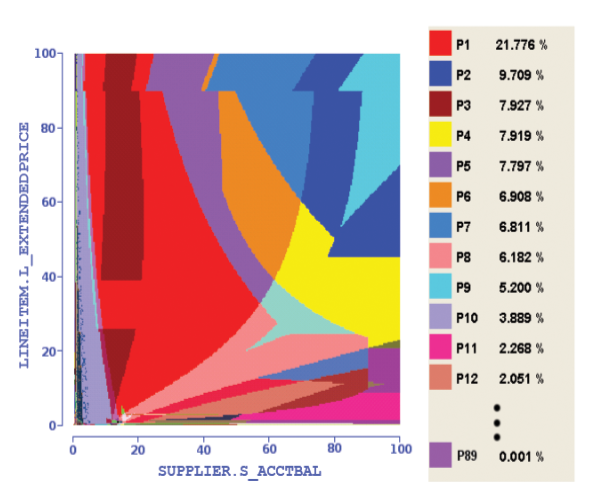
\includegraphics[scale=0.6]{Images/Picasso.png}
  \caption[A query plan visualisation done by Picasso]{A query plan
    visualisation done by Picasso, image taken
    from~\cite{haritsa_2010_picasso_tpdqov}.}\label{fig:picasso}
\end{figure}

Finally, on a more practical note Lahdenmäki  et\ al.\ describe of how to
identify queries where the selected access path is bad, and how to solve the
problem~\cite{lahdenmaki_2005_relational_rdidatodossea}. The book gives a
thorough introduction to many important aspects of the database and the chapter
``Optimizers Are Not Perfect'' focuses on incorrect cardinality estimates and
other common query optimizer errors.

\section{Bad statistics and cardinality estimates}
In~\cite{ioannidis_1991_propagation_otpoeitsojr} Ionnidis  et\ al.\ develop a
framework to study how cardinality estimate errors propagate in queries. Their
results indicate that the error increases exponentially with the number joins.

There are two different methods of improving how optimizers handle cardinality
estimation:
\begin{itemize}
\item Reducing the effect of incorrect estimations by making plans more
  \textit{robust}, which means they perform better over large regions of the
  search space;
\item Or by improving the estimations.
\end{itemize}

\subsection{Improving robustness}
Harish et\ al.\ present a way to make plans more robust by allowing the
optimizer to select the most robust plan that is not ``too slow'' compared to
the calculated optimal path.~\cite{harish_2008_identifying_irptpdr}. They
develop an external tool for this purpose and find that the tool indeed does
improve performance by reducing the effect of selectivity errors.

A similar study is done by Abhirama et\ al.\ but they implement the selection
directly in the PostgreSQL query
optimizer~\cite{abhirama_2010_stability_otsopcatcops}. Their results agree with
those found by Harish  et\ al.\ in that the performance is improved. The results
they present show that robut plans often reduced the adverse effects of
selectivity errors by more than two-thirds, while only providing a minor overhead in
terms of time and memory.

\subsection{Improving cardinality estimates}\label{sec:improving_cardinality_estimates}
The most studied problem of cardinality estimate is that of finding the right
balance between calculation time, memory overhead and correctness. One common
method used in current state-of-the-art databases is histograms that assume
attributes are independent of each other, an assumption that often is not
correct~\cite{ioannidis_2003_history_thoha}. Recent studies have been done to
find alternatives method that do not assume independence.

Tzoumas et\ al.\ present one method that instead of the usual one-dimensional
statistical summary, saves it as a small, two-dimensional
distribution~\cite{tzoumas_2011_lightweight_lgmfsewia}. Their results show a
small overhead with selectivity estimates being better by an order of magnitude.

In~\cite{yu_2013_cs2_candsfqea} Yu et\ al.\ develop a  method called
\textit{Correlated Sampling} that does not sample randomly, but rather save
correlated sample tuples that retain join relationships. They further develop an
estimator, called reverse estimator, that use correlated sample tuples for query
estimation. Their results indicate that the estimator is fast to construct and
provides better estimations than existing methods.

In~\cite{vengerov_2015_join_jsestfc} Vengerov et\ al.\ once again study
Correlated Sampling, but improve on it by allowing it to only make a single pass
over the data. They compare the algorithm to two other sampling approaches
(Independent Bernoulli Sampling and End-Biased Sampling, which is described
in~\cite{estan_2006_end_esfjce}) and find Correlated Sampling to provide the best
estimates in a large range of situations.

\section{Improving operators}
In~\cite{muller_2015_cache_cahis} Müller  et\ al.\ study the two implementations
of relational operators: hashing and sorting (more about these in
Section~\ref{sec:opimpl}). Their study find that the two paradigms are in terms
of cache efficiency actually the same and from this observation develop a
relational aggregation algorithm that outperform state-of-the-art methods by up
to 3.7 times.

A problem described in~\cite{leis_2015_how_hgaqor} is that the optimizer tends
to pick nested-loop joins (more about these in Section~\ref{sec:nestedloopjoin})
even though they provide a high risk but only a very small payoff.
In~\cite{graefe_2011_generalized_agja} Goetz Graefe provides a generalized join
algorithm that can replace both merge joins and hash joins in databases, thus
avoiding the danger of an incorrectly chosen join algorithm during query optimization.
